\documentclass[11pt,a4]{article}
\usepackage{graphicx}
\usepackage{xcolor}
\usepackage{tabularx}
\usepackage{amsmath}
\usepackage[utf8]{inputenc}
\usepackage[T1]{fontenc}
\usepackage[french]{babel}
\usepackage{hyperref}
\usepackage{pdfpages}
\pagestyle{empty}
\topmargin -2cm
\textheight 22cm
\textwidth 15 cm
\oddsidemargin 0.46cm
\evensidemargin 0.46cm
\parskip=0.2 true cm
\headsep 2.cm

\begin{document}

% en-tête

\begin{figure}
    \begin{minipage}[c]{.06\linewidth}
        
\includegraphics[width = 3.5 true cm]{../phast-logo.png}
    \end{minipage} \hfill
    \begin{minipage}[c]{.66\linewidth}
        \begin{center}
            {\bf \Large Campagne 2019 de recrutement \\ sur contrat doctoral}
        \end{center}
    \end{minipage}
    \begin{minipage}[c]{.06\linewidth}
        
\includegraphics[width = 3.5 true cm]{../UdL-logo.png}
    \end{minipage}
\end{figure}

\begin{center}
    {\bf \Large Dossier de candidature -- Partie A (CV académique)}
\end{center}

% Photo candidat

\begin{center}
    \begin{tabular}{|m{12cm}|m{4cm}|} \hline
    \vspace{1.5cm} {\hskip 5 true cm} \textsc{Nicolas} Nora \vspace{1.5cm}
    & \hspace{.7cm} 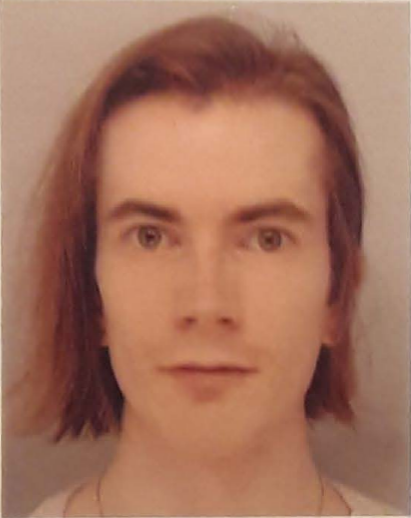
\includegraphics[width = 2 cm]{../nora_pid.png}
        \\ \hline
    \end{tabular}
\end{center}

% Informations

\noindent {\bf Adresse personnelle :} 
3 boulevard des Brotteaux, 69006 Lyon

\vglue 0.5 true cm

\noindent {\bf Téléphone portable :}
06 06 53 50 92

\vglue 0.5 true cm

\noindent {\bf Adresse électronique :}
\href{mailto:nora.nicolas@ens-lyon.fr}{nora.nicolas@ens-lyon.fr}

\vglue 0.5 true cm

\noindent {\bf Libellé du master :}
ENS de Lyon, Master Physique, Concepts et Applications

\vglue 0.5 true cm

\noindent {\bf Nom et adresse électronique du responsable pouvant attester du classement :}
\textsc{Bartolo} Denis, \href{mailto:denis.bartolo@ens-lyon.fr}{denis.bartolo@ens-lyon.fr}

\vglue 0.5 true cm

\noindent {\bf Cursus académique :} \\ Pour l'année universitaire en cours, seuls les résultats
partiels sont demandés.

\begin{center}
    \begin{tabular}{|c|c|c|c|c|c|} \cline{1-6}
        Année     & Formation               & Établissement & Moyenne & Rang & Effectifs \\ \hline
        2018-2019 & M2 Recherche            & ENS de Lyon   & 11.3    &      & 48 \\ \hline
        2017-2018 & M2 FEADéP -- Agrégation & ENS de Lyon   & 14.6    & 9    & 23 \\ \hline
        2016-2017 & M1 Recherche            & ENS de Lyon   & 12.5    & 56   & 61 \\ \hline
        2015-2016 & L3 Physique             & ENS de Lyon   & 15.6    & 19   & 50 \\ \hline
    \end{tabular}
\end{center}

\newpage
\noindent {\bf Lettre de motivation (max 15 lignes) :}\\

Actuellement en Master 2 de physique à l'ENS de Lyon après l'obtention de l'agrégation de physique,
je souhaite maintenant vivement continuer mon parcours par une thèse en cosmologie observationnelle.
Cette matière me passionne depuis mon plus jeune âge et a été la source de ma motivation et de mes
efforts qui m'ont permis de poursuivre une formation universitaire d'excellence, malgré une
situation personnelle parfois difficile. 

Au cours de ces années, j'ai découvert de nombreux aspects de la physique par mes enseignements
divers et par mes stages. Ceux-ci ont toujours renouvelé mon engouement pour cette discipline et
j'ai particulièrement apprécié mettre mes connaissances académiques à profit de nouvelles
recherches. À ce titre, apprendre différents langages de programmation pour effectuer ces travaux
furent de très bonnes expériences. J'ai alors compris les attentes inhérentes à un travail de
recherche sur le long terme, ainsi que la nécessité de faire partie d'un groupe dynamique et aux
méthodes de travail rigoureuses. Ces stages m'ont donc confirmé mon désir de faire de la recherche. 

Le sujet de recherche proposé par l'équipe de cosmologie de l'IPNL allie tout ce qui m'est cher :
théorie, étude et traitement de données sur un sujet passionnant au carrefour de nombreuses branches
de la physique. La perspective de réaliser une thèse dans ce domaine est donc la concrétisation de
mon parcours riche en expériences et de ma préférence initiale.

\vglue 7 true cm

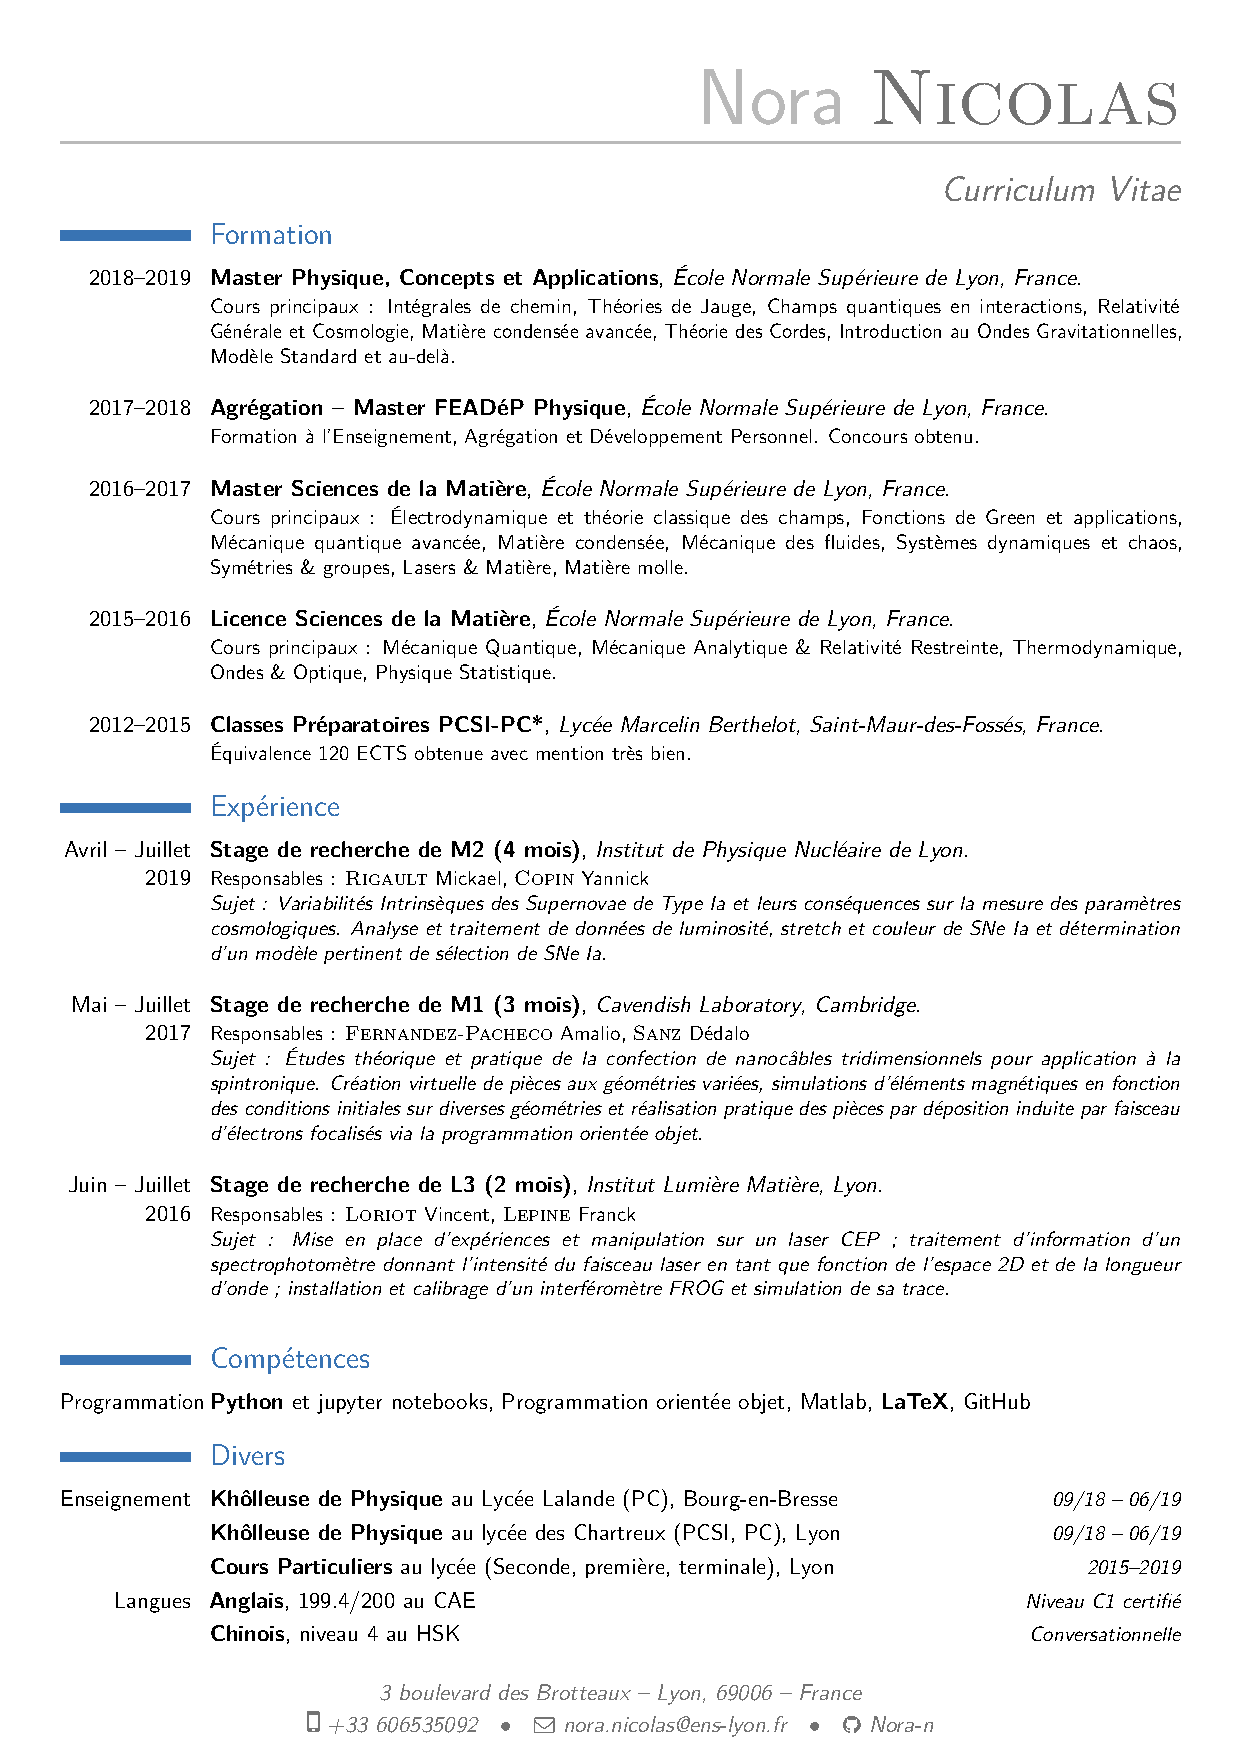
\includepdf[pages=-]{CV_Nora_NICOLAS_2019_French.pdf}

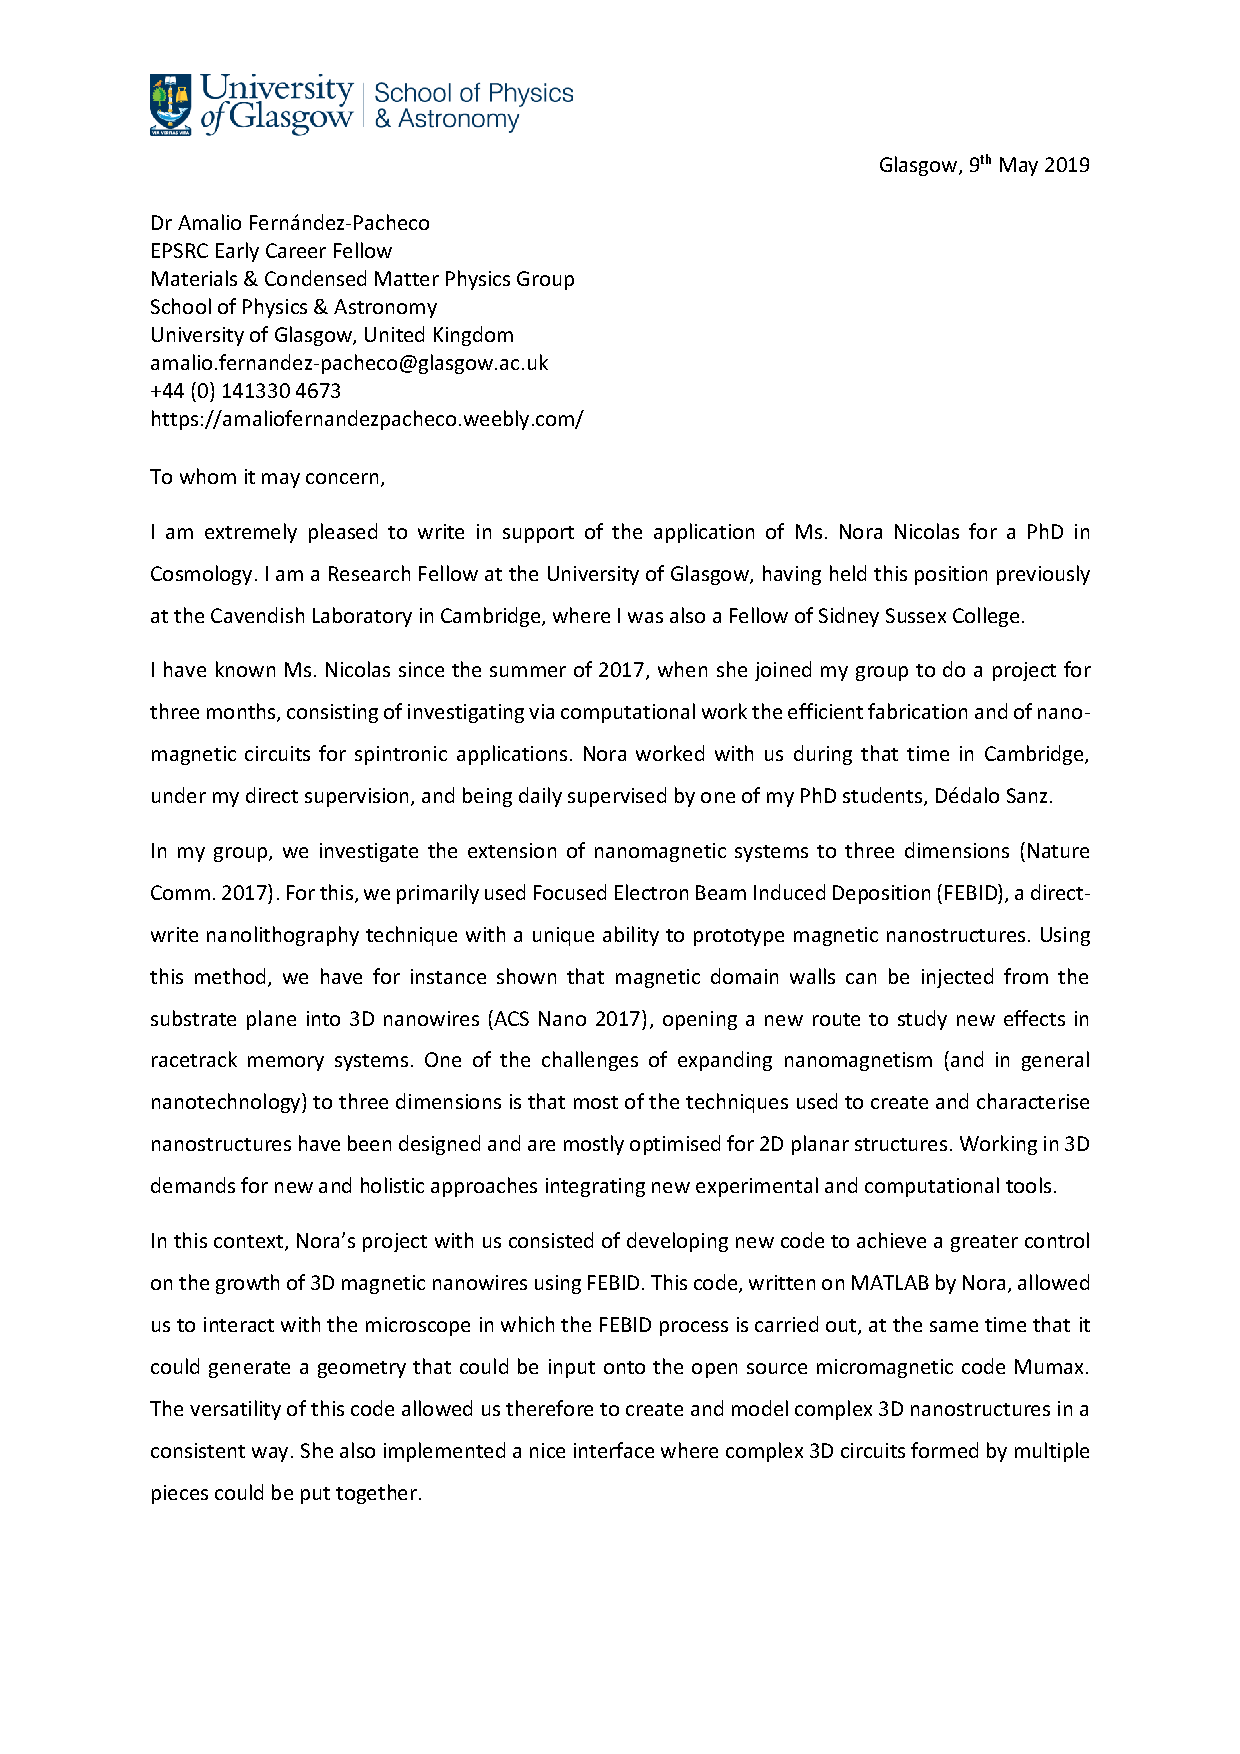
\includepdf[pages=-]{References/Amalio_reference_letter}
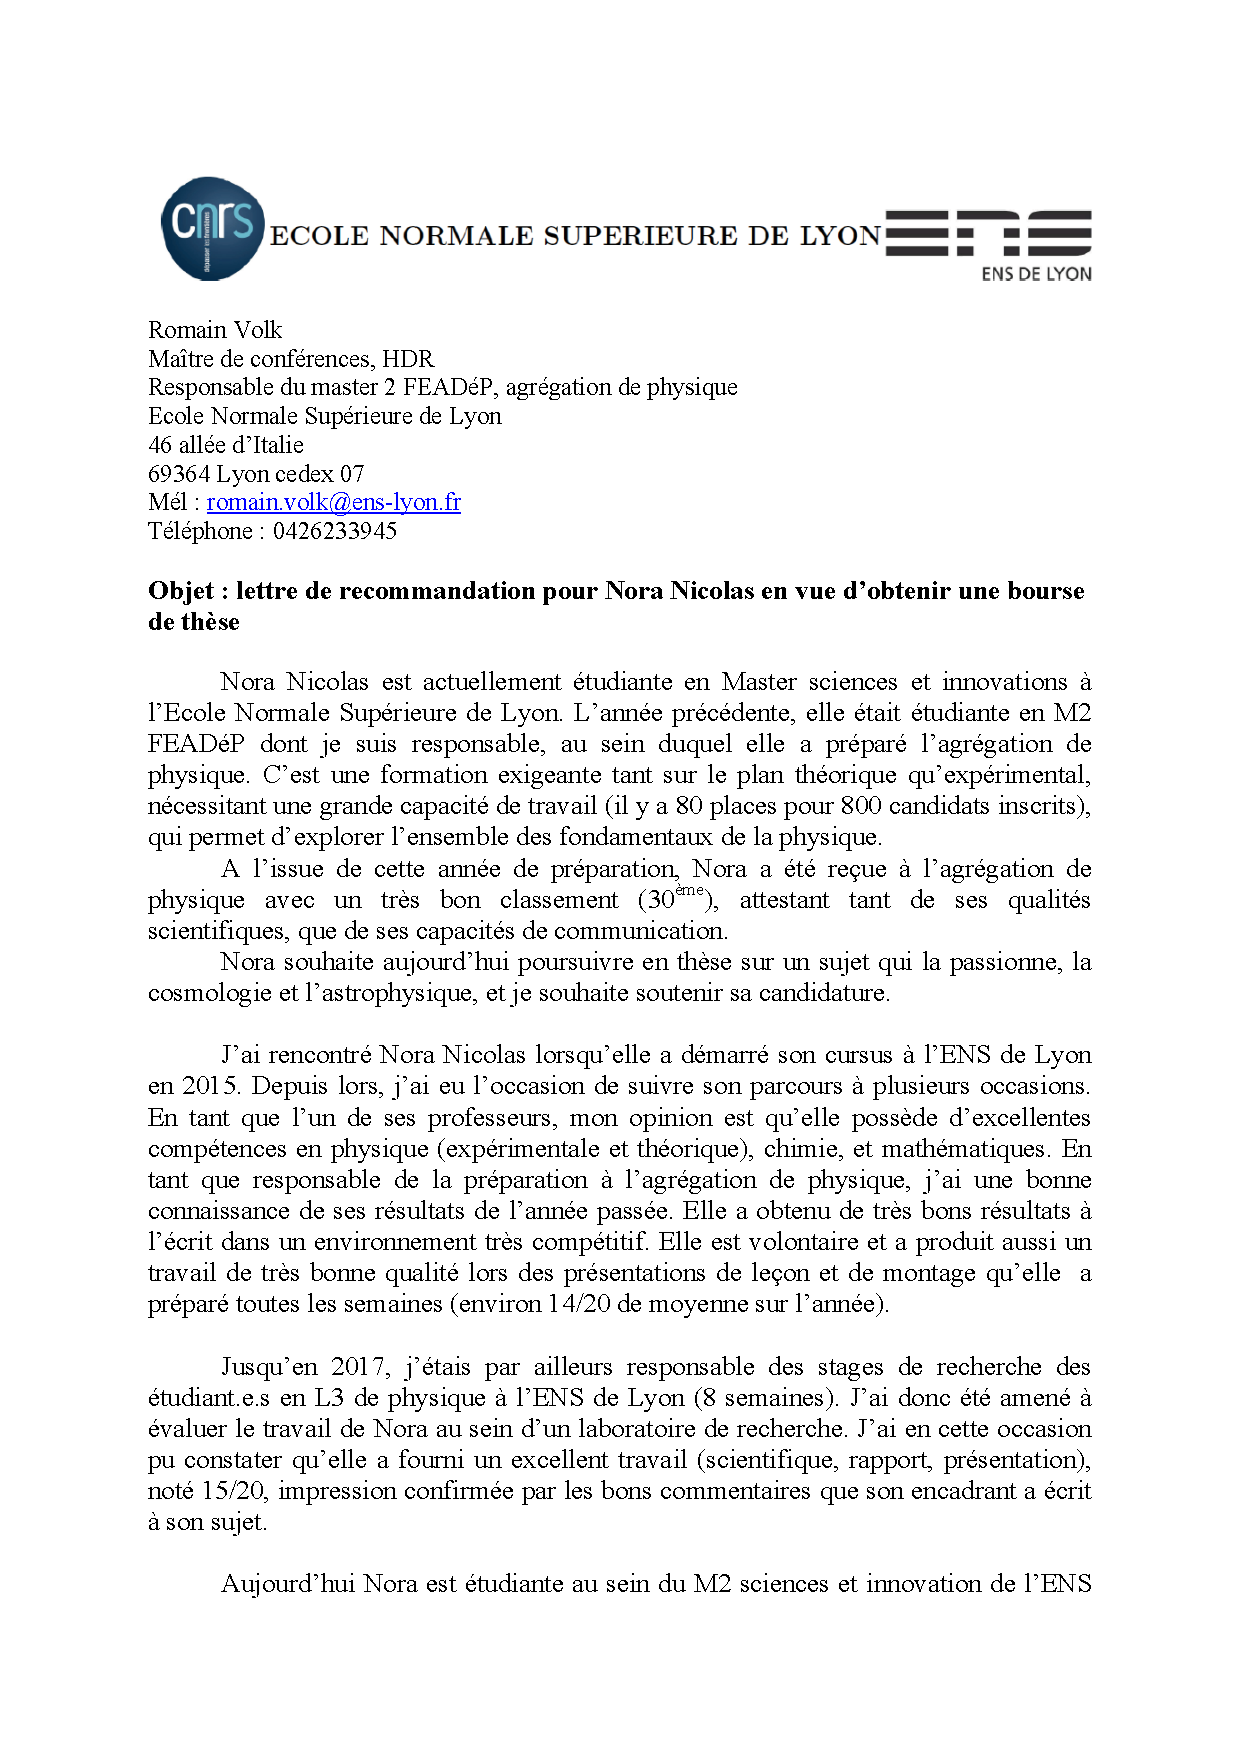
\includepdf[pages=-]{References/Volk_reference_letter}
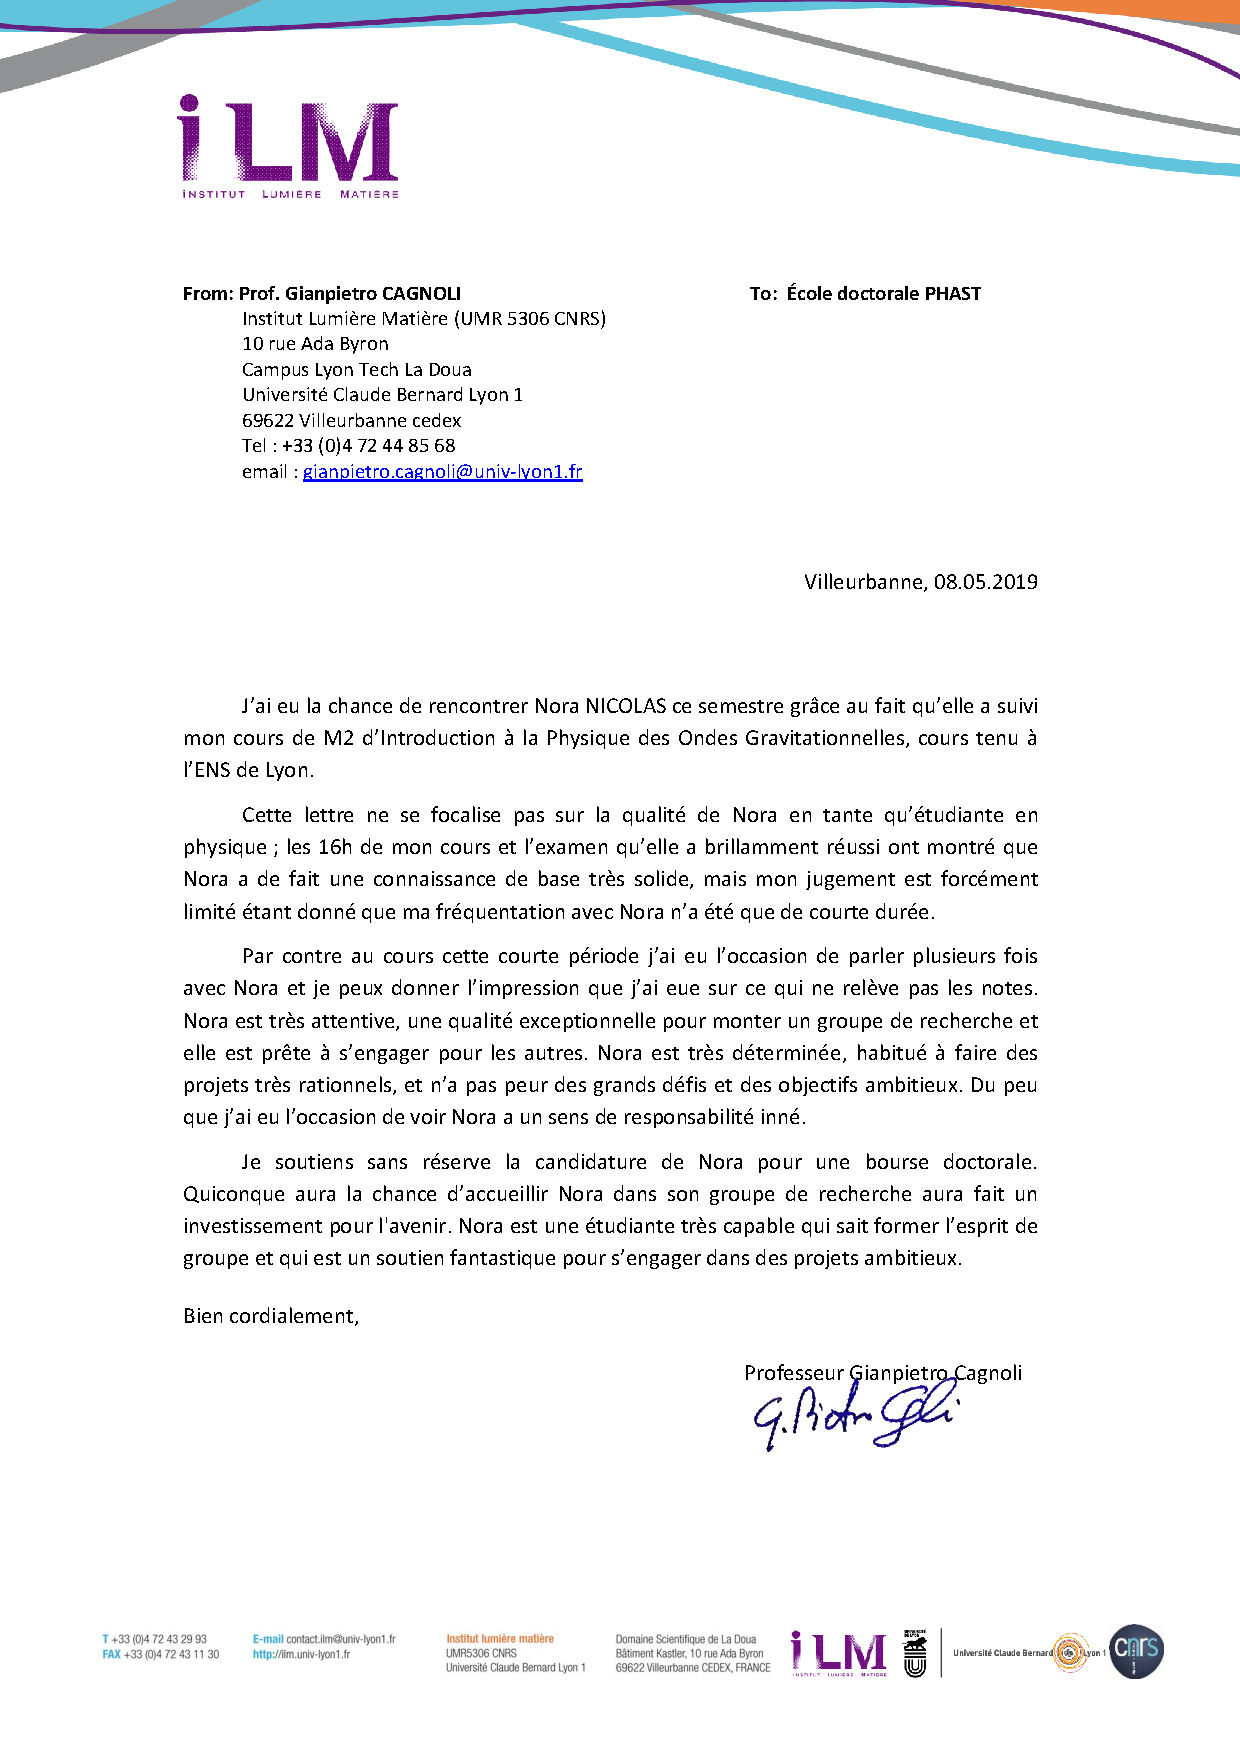
\includepdf[pages=-]{References/Cagnoli_reference_letter}

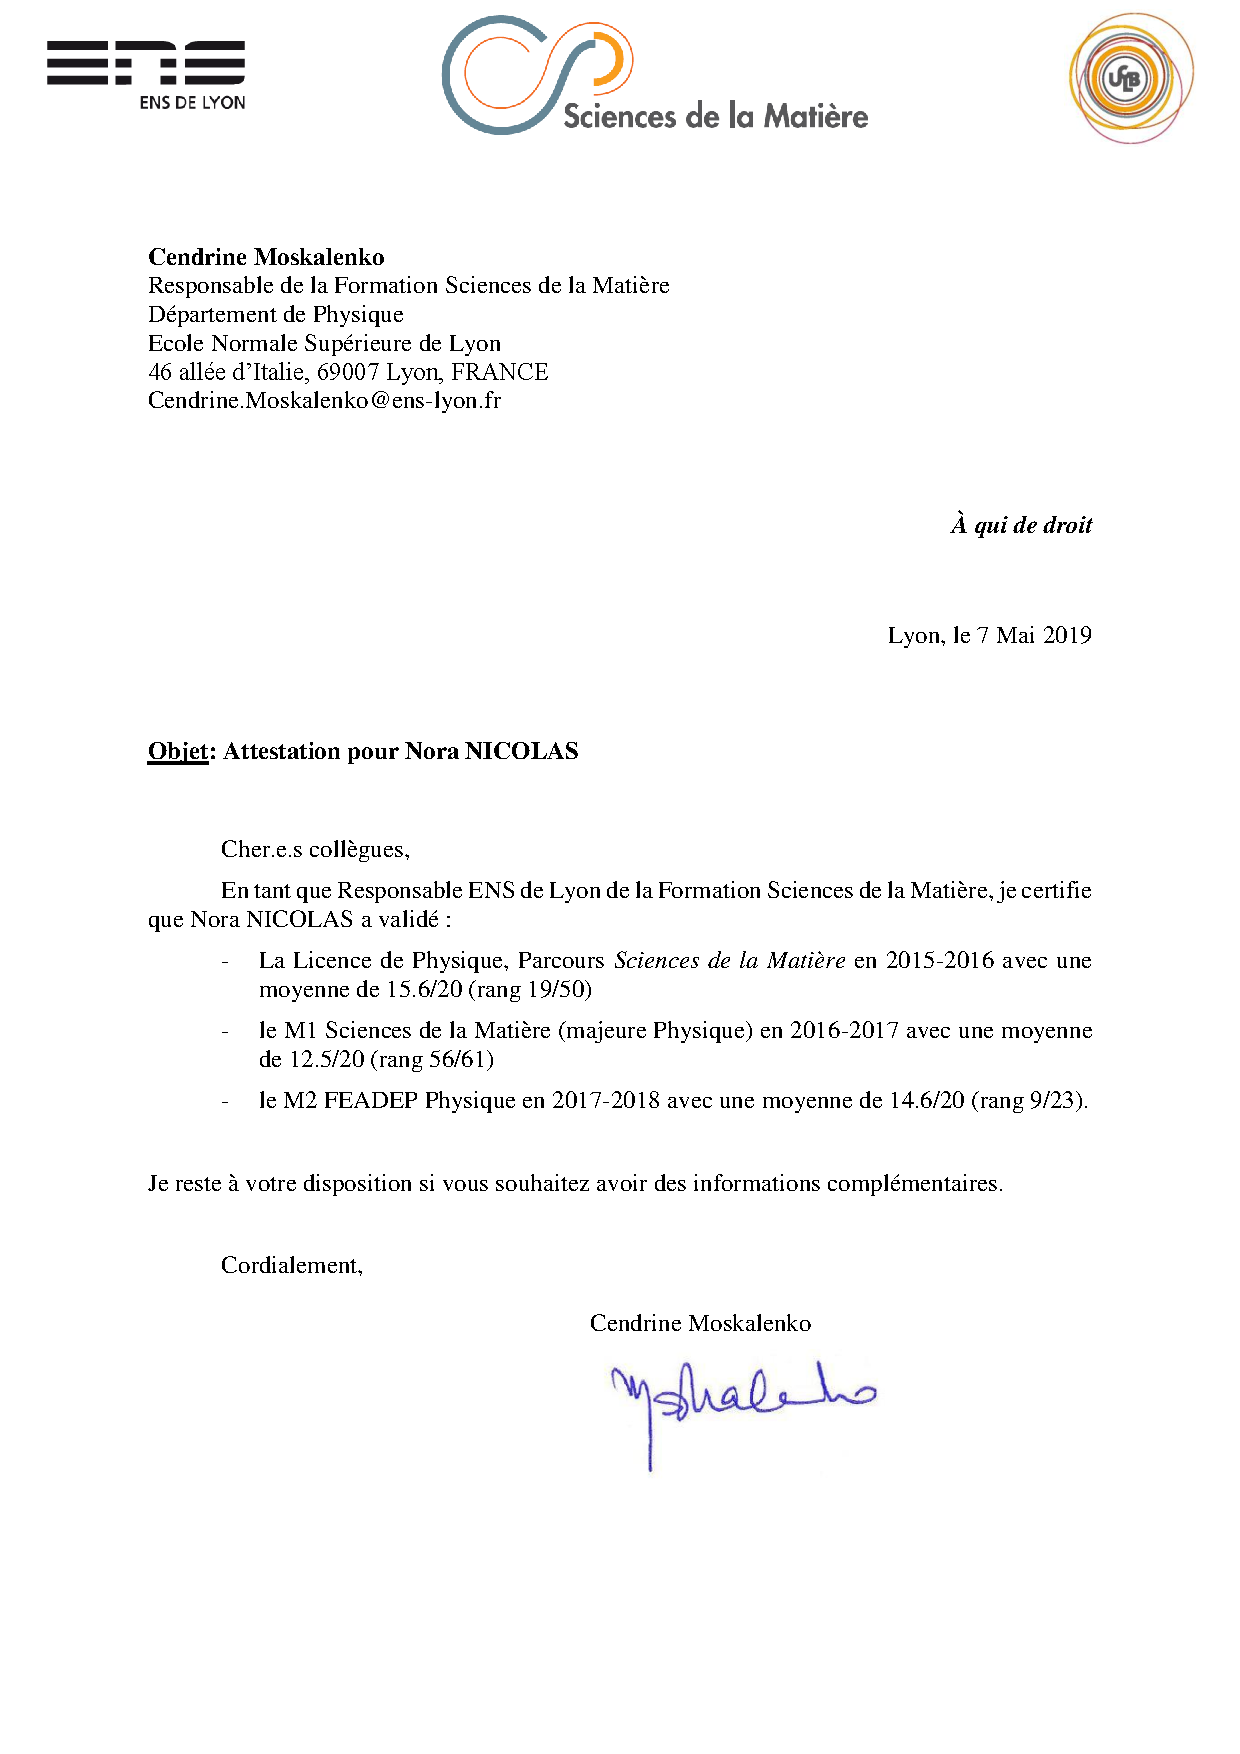
\includepdf[pages=-]{Notes/attestation.pdf}
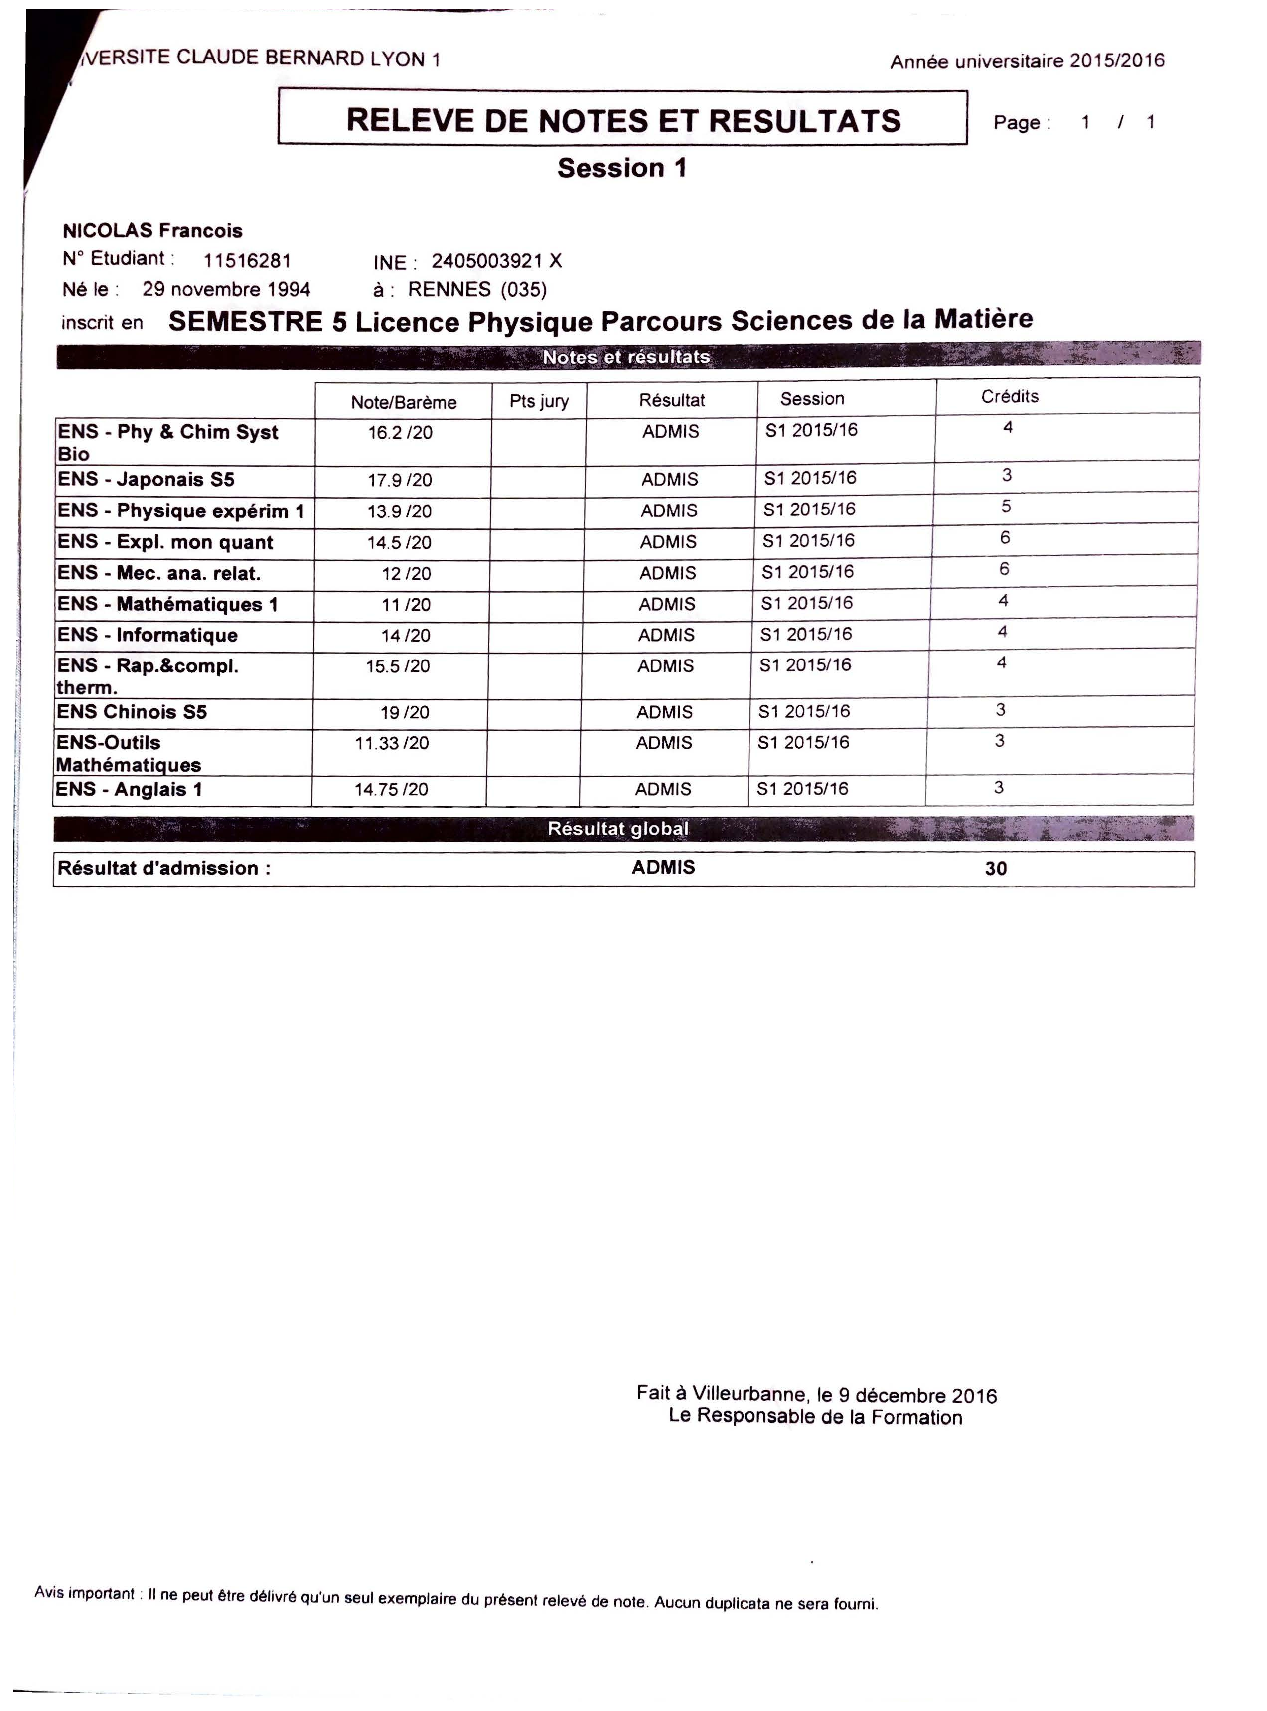
\includepdf[pages=-]{Notes/notes_L3.pdf}
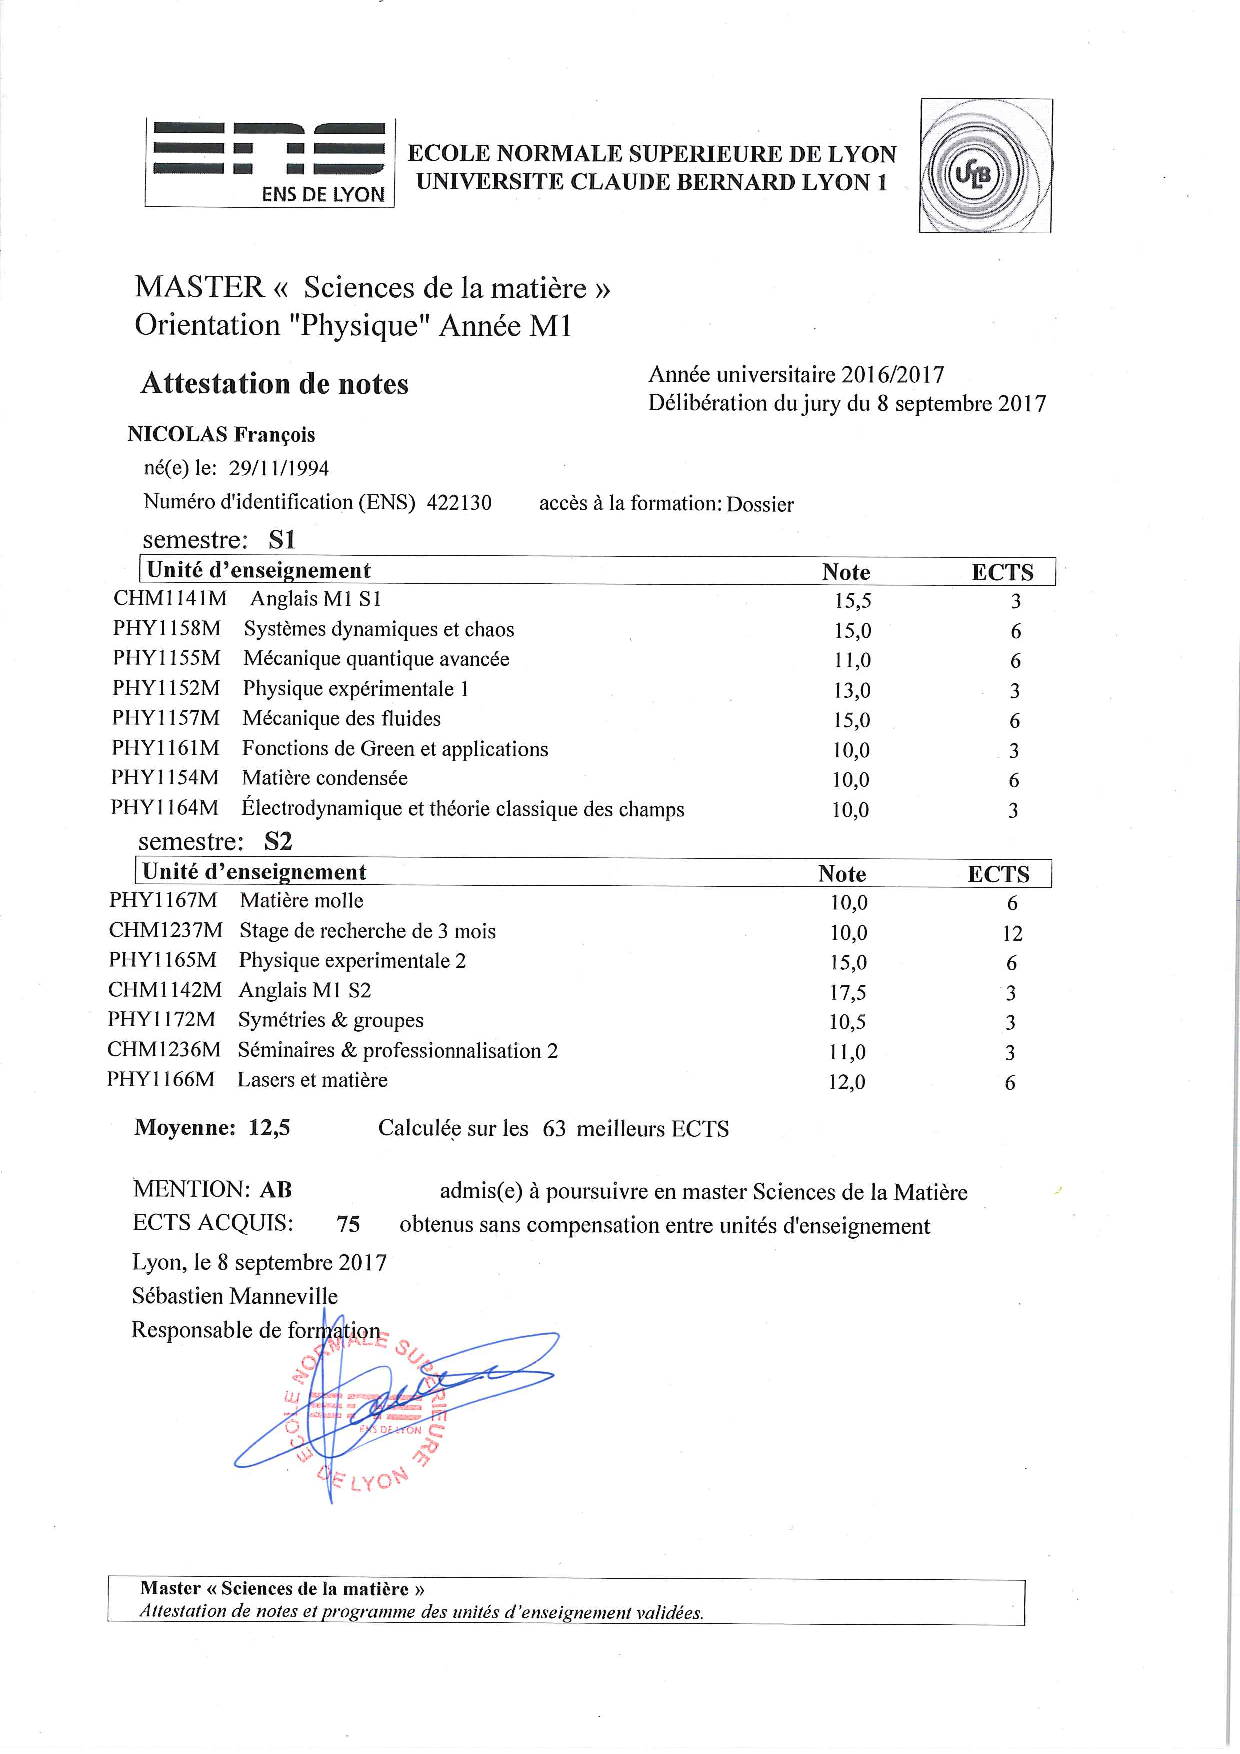
\includepdf[pages=-]{Notes/notes_M1.pdf}
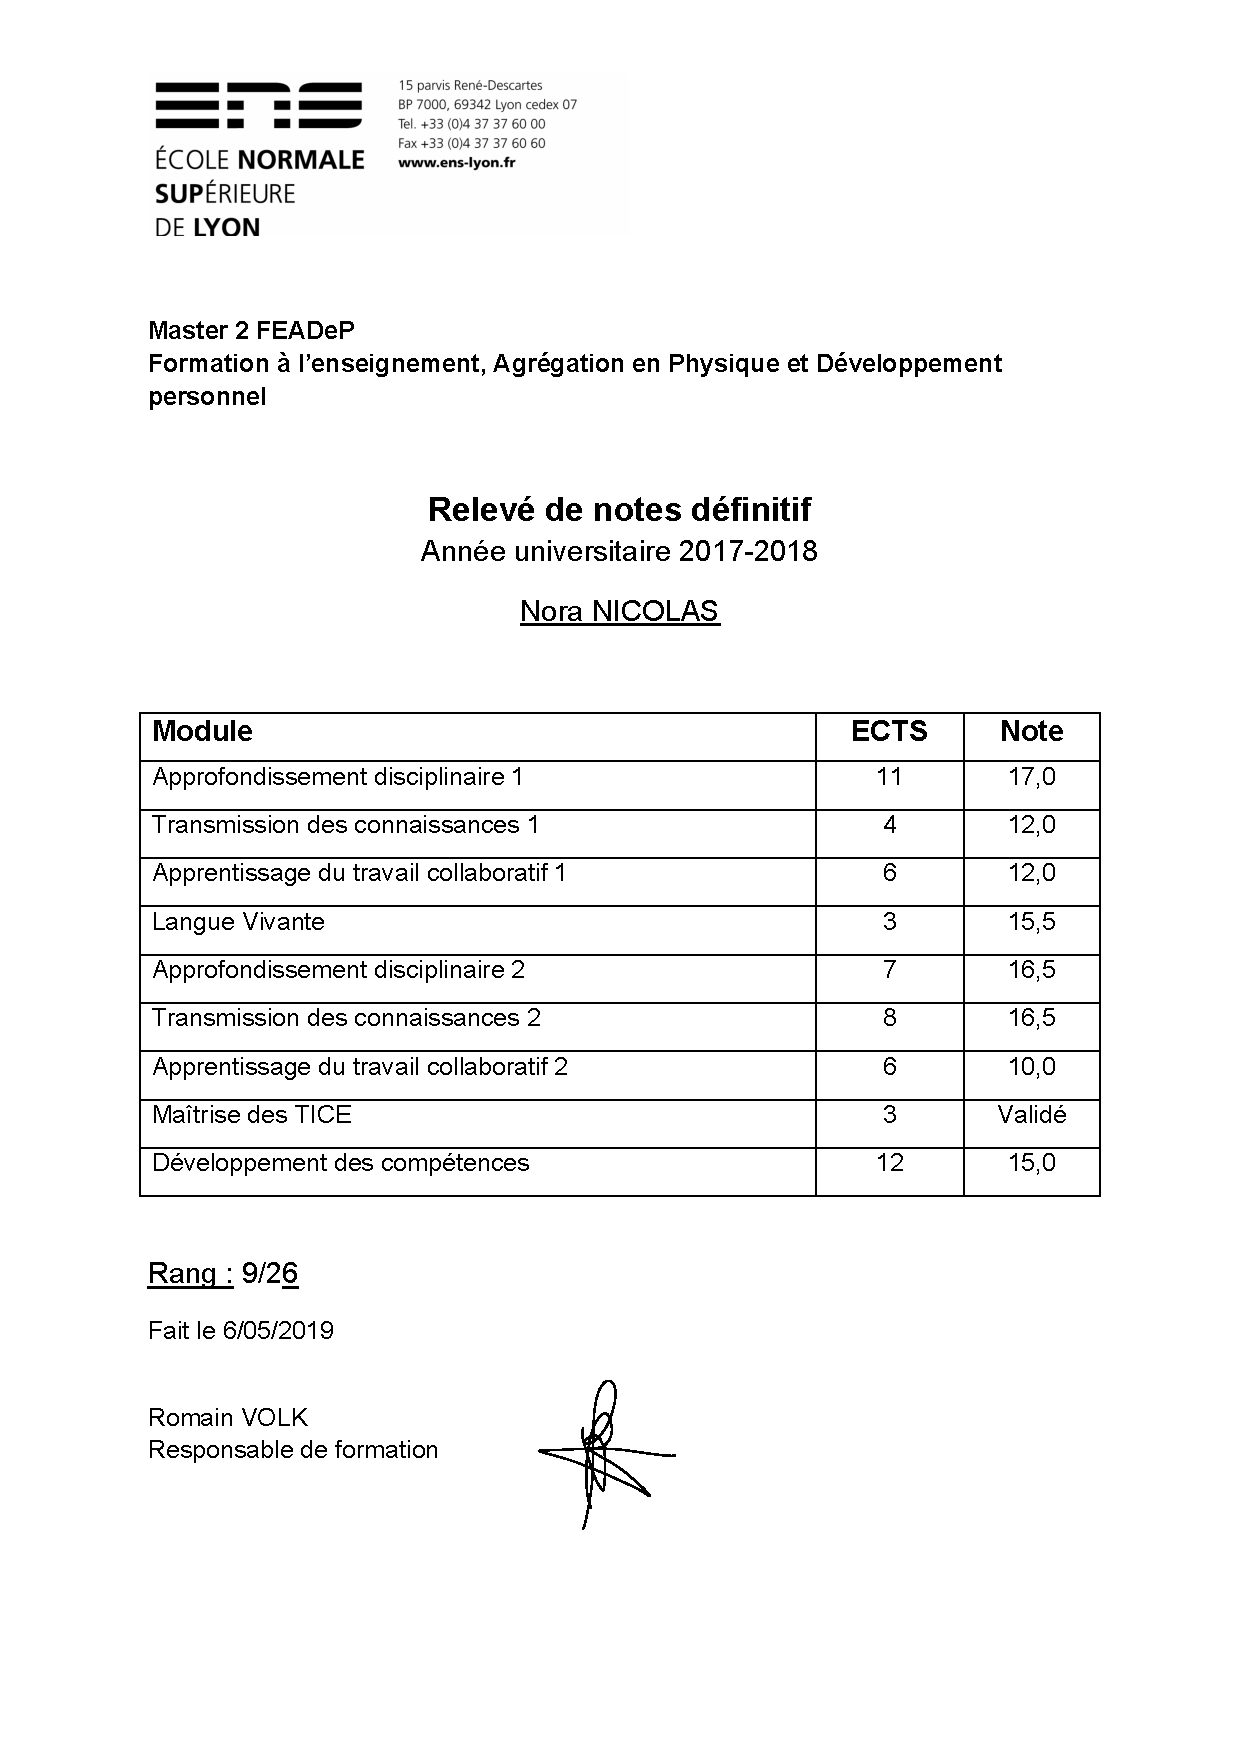
\includepdf[pages=-]{Notes/notes_agreg.pdf}
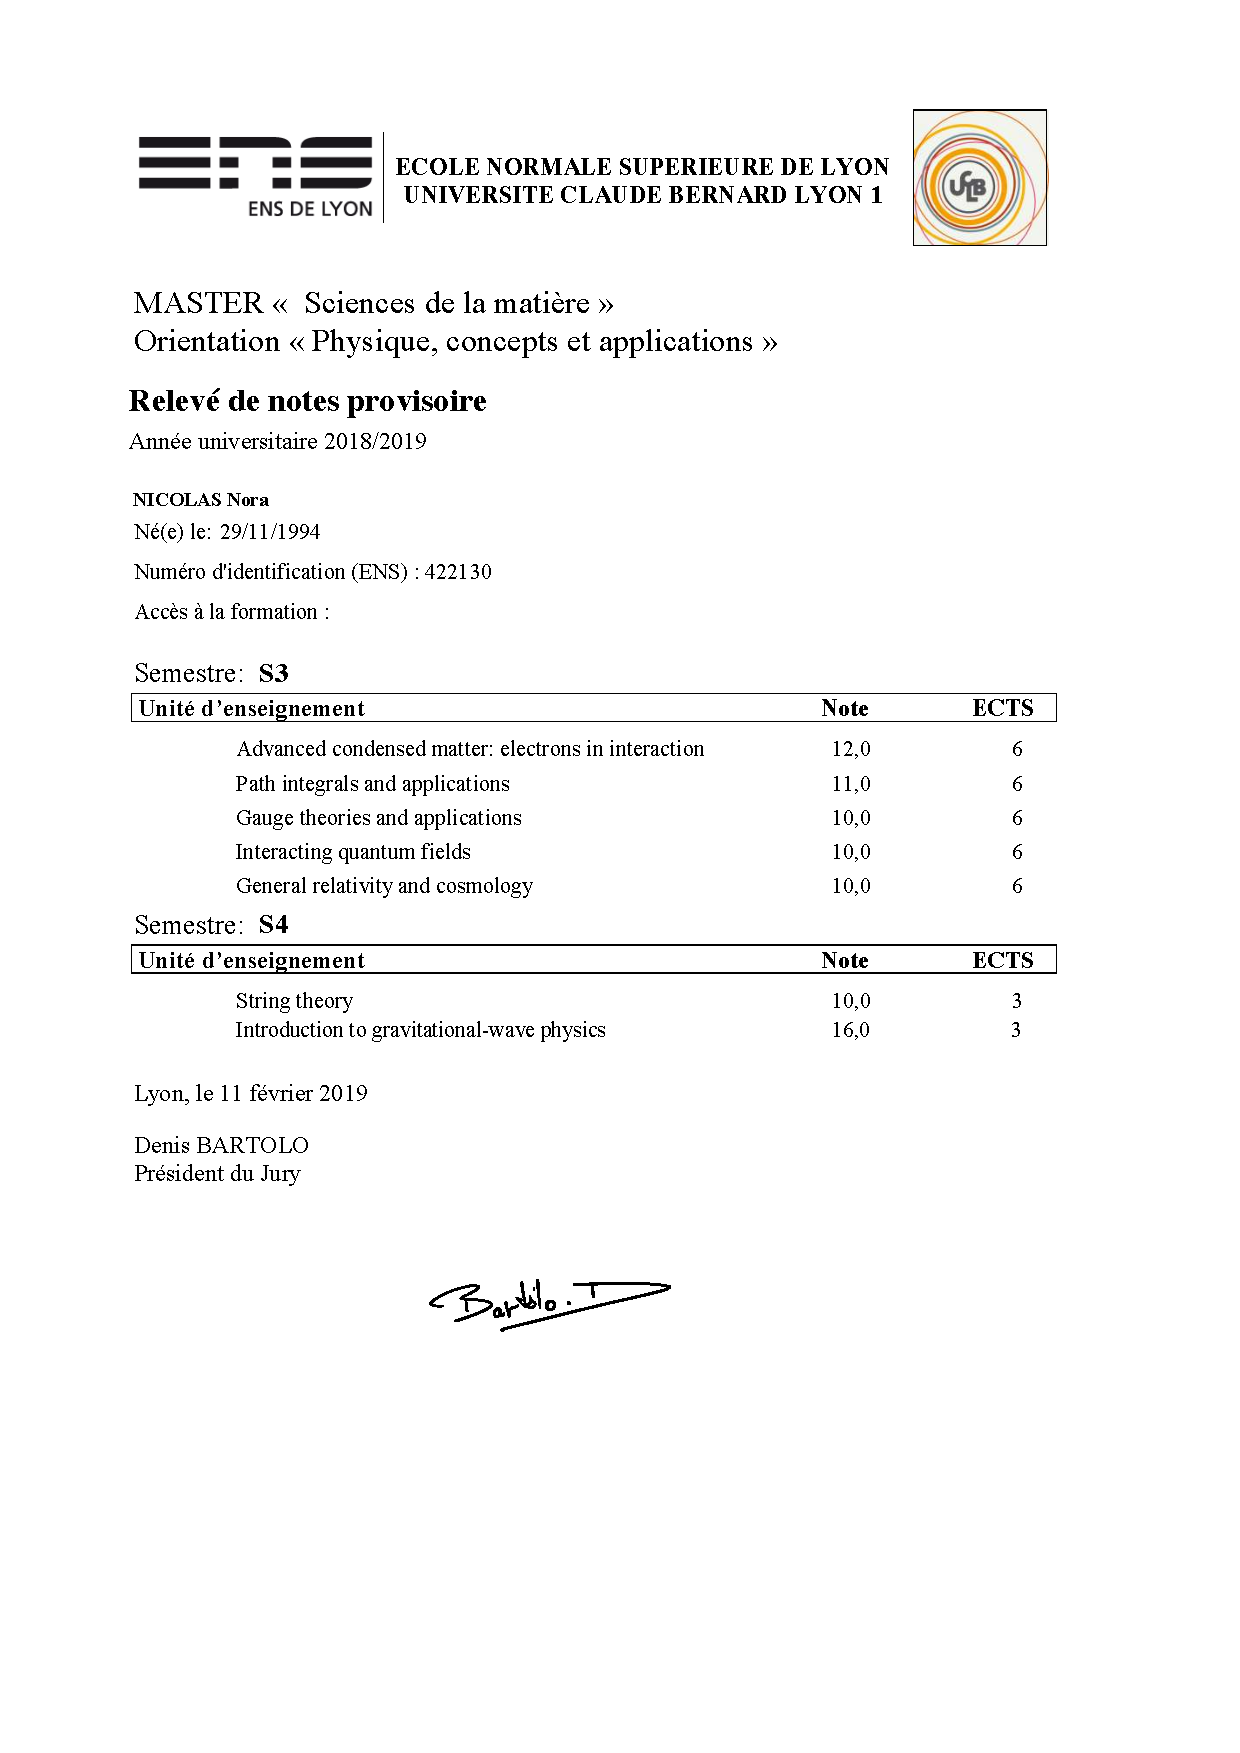
\includepdf[pages=-]{Notes/notes_M2.pdf}

\end{document}
